%%%%%%%%%%%%%%%%%%%%%%%%%%%%%%%%%%%%%%%%%
% Beamer Presentation
% LaTeX Template
% Version 2.0 (March 8, 2022)
%
% This template originates from:
% https://www.LaTeXTemplates.com
%
% Author:
% Vel (vel@latextemplates.com)
%
% License:
% CC BY-NC-SA 4.0 (https://creativecommons.org/licenses/by-nc-sa/4.0/)
%
%%%%%%%%%%%%%%%%%%%%%%%%%%%%%%%%%%%%%%%%%

%----------------------------------------------------------------------------------------
%	PACKAGES AND OTHER DOCUMENT CONFIGURATIONS
%----------------------------------------------------------------------------------------

\documentclass[
	11pt, % Set the default font size, options include: 8pt, 9pt, 10pt, 11pt, 12pt, 14pt, 17pt, 20pt
	%t, % Uncomment to vertically align all slide content to the top of the slide, rather than the default centered
	%aspectratio=169, % Uncomment to set the aspect ratio to a 16:9 ratio which matches the aspect ratio of 1080p and 4K screens and projectors
]{beamer}

\graphicspath{{Images/}{./}} % Specifies where to look for included images (trailing slash required)

\usepackage{booktabs} % Allows the use of \toprule, \midrule and \bottomrule for better rules in tables

%----------------------------------------------------------------------------------------
%	SELECT LAYOUT THEME
%----------------------------------------------------------------------------------------

% Beamer comes with a number of default layout themes which change the colors and layouts of slides. Below is a list of all themes available, uncomment each in turn to see what they look like.

%\usetheme{default}
%\usetheme{AnnArbor}
%\usetheme{Antibes}
%\usetheme{Bergen}
%\usetheme{Berkeley}
%\usetheme{Berlin}
%\usetheme{Boadilla}
%\usetheme{CambridgeUS}
%\usetheme{Copenhagen}
%\usetheme{Darmstadt}
%\usetheme{Dresden}
%\usetheme{Frankfurt}
%\usetheme{Goettingen}
%\usetheme{Hannover}
%\usetheme{Ilmenau}
%\usetheme{JuanLesPins}
%\usetheme{Luebeck}
\usetheme{Madrid}
%\usetheme{Malmoe}
%\usetheme{Marburg}
%\usetheme{Montpellier}
%\usetheme{PaloAlto}
%\usetheme{Pittsburgh}
%\usetheme{Rochester}
%\usetheme{Singapore}
%\usetheme{Szeged}
%\usetheme{Warsaw}

%----------------------------------------------------------------------------------------
%	SELECT COLOR THEME
%----------------------------------------------------------------------------------------

% Beamer comes with a number of color themes that can be applied to any layout theme to change its colors. Uncomment each of these in turn to see how they change the colors of your selected layout theme.

%\usecolortheme{albatross}
%\usecolortheme{beaver}
%\usecolortheme{beetle}
%\usecolortheme{crane}
%\usecolortheme{dolphin}
%\usecolortheme{dove}
%\usecolortheme{fly}
%\usecolortheme{lily}
%\usecolortheme{monarca}
%\usecolortheme{seagull}
%\usecolortheme{seahorse}
%\usecolortheme{spruce}
%\usecolortheme{whale}
%\usecolortheme{wolverine}

%----------------------------------------------------------------------------------------
%	SELECT FONT THEME & FONTS
%----------------------------------------------------------------------------------------

% Beamer comes with several font themes to easily change the fonts used in various parts of the presentation. Review the comments beside each one to decide if you would like to use it. Note that additional options can be specified for several of these font themes, consult the beamer documentation for more information.

\usefonttheme{default} % Typeset using the default sans serif font
%\usefonttheme{serif} % Typeset using the default serif font (make sure a sans font isn't being set as the default font if you use this option!)
%\usefonttheme{structurebold} % Typeset important structure text (titles, headlines, footlines, sidebar, etc) in bold
%\usefonttheme{structureitalicserif} % Typeset important structure text (titles, headlines, footlines, sidebar, etc) in italic serif
%\usefonttheme{structuresmallcapsserif} % Typeset important structure text (titles, headlines, footlines, sidebar, etc) in small caps serif

%------------------------------------------------

%\usepackage{mathptmx} % Use the Times font for serif text
\usepackage{palatino} % Use the Palatino font for serif text

%\usepackage{helvet} % Use the Helvetica font for sans serif text
\usepackage[default]{opensans} % Use the Open Sans font for sans serif text
%\usepackage[default]{FiraSans} % Use the Fira Sans font for sans serif text
%\usepackage[default]{lato} % Use the Lato font for sans serif text

%----------------------------------------------------------------------------------------
%	SELECT INNER THEME
%----------------------------------------------------------------------------------------

% Inner themes change the styling of internal slide elements, for example: bullet points, blocks, bibliography entries, title pages, theorems, etc. Uncomment each theme in turn to see what changes it makes to your presentation.

%\useinnertheme{default}
\useinnertheme{circles}
%\useinnertheme{rectangles}
%\useinnertheme{rounded}
%\useinnertheme{inmargin}

%----------------------------------------------------------------------------------------
%	SELECT OUTER THEME
%----------------------------------------------------------------------------------------

% Outer themes change the overall layout of slides, such as: header and footer lines, sidebars and slide titles. Uncomment each theme in turn to see what changes it makes to your presentation.

%\useoutertheme{default}
%\useoutertheme{infolines}
%\useoutertheme{miniframes}
%\useoutertheme{smoothbars}
%\useoutertheme{sidebar}
%\useoutertheme{split}
%\useoutertheme{shadow}
%\useoutertheme{tree}
%\useoutertheme{smoothtree}

%\setbeamertemplate{footline} % Uncomment this line to remove the footer line in all slides
%\setbeamertemplate{footline}[page number] % Uncomment this line to replace the footer line in all slides with a simple slide count

%\setbeamertemplate{navigation symbols}{} % Uncomment this line to remove the navigation symbols from the bottom of all slides

\setbeamertemplate{bibliography item}[text]
%----------------------------------------------------------------------------------------
%	PRESENTATION INFORMATION
%----------------------------------------------------------------------------------------

\title[Digital Tools for Finance]{Markowitz-Optimal Portfolio \\ Under Inflation in China} % The short title in the optional parameter appears at the bottom of every slide, the full title in the main parameter is only on the title page

\subtitle{} % Presentation subtitle, remove this command if a subtitle isn't required

\author[Zhang, Hu, Lin, Han]{Yunpeng Zhang\and Zhiying Hu\and Xuanzhi Lin\and Zelong Han} % Presenter name(s), the optional parameter can contain a shortened version to appear on the bottom of every slide, while the main parameter will appear on the title slide

\institute{University of Zurich} % Your institution, the optional parameter can be used for the institution shorthand and will appear on the bottom of every slide after author names, while the required parameter is used on the title slide and can include your email address or additional information on separate lines

\date[December 18, 2022]{December 18, 2022} % Presentation date or conference/meeting name, the optional parameter can contain a shortened version to appear on the bottom of every slide, while the required parameter value is output to the title slide

%----------------------------------------------------------------------------------------

\begin{document}

%----------------------------------------------------------------------------------------
%	TITLE SLIDE
%----------------------------------------------------------------------------------------

\begin{frame}
	\titlepage % Output the title slide, automatically created using the text entered in the PRESENTATION INFORMATION block above
\end{frame}

%----------------------------------------------------------------------------------------
%	TABLE OF CONTENTS SLIDE
%----------------------------------------------------------------------------------------

% The table of contents outputs the sections and subsections that appear in your presentation, specified with the standard \section and \subsection commands. You may either display all sections and subsections on one slide with \tableofcontents, or display each section at a time on subsequent slides with \tableofcontents[pausesections]. The latter is useful if you want to step through each section and mention what you will discuss.

\begin{frame}
	\frametitle{Presentation Overview} % Slide title, remove this command for no title
	
	\tableofcontents % Output the table of contents (all sections on one slide)
	%\tableofcontents[pausesections] % Output the table of contents (break sections up across separate slides)
\end{frame}

%------------------------------------------------
%	PRESENTATION BODY SLIDES
%------------------------------------------------
%------------------------------------------------
%------------------------------------------------
\section{Introduction} % Sections are added in order to organize your presentation into discrete blocks, all sections and subsections are automatically output to the table of contents as an overview of the talk but NOT output in the presentation as separate slides
\subsection{Background}
%------------------------------------------------
\begin{frame}
\frametitle{Introduction}
\framesubtitle{Background}
\begin{itemize}
\item Global inflation has reached its \textcolor{blue}{highest level} since 2008 in recent years due to the shock of covid-19, supply chain disruptions, and increasingly tense international conditions.\\
\bigskip
\item Inflation implies a prolonged period of rising price levels, which leads to  a \textcolor{blue}{contraction in the real value of assets}.\\
\bigskip
\item The erosion of the real return of a portfolio caused by inflation is one of the fundamental risks faced by investors in financial markets.\\
\end{itemize}
\end{frame}
%------------------------------------------------
%------------------------------------------------
\subsection{Literature Review}
\begin{frame}
\frametitle{Introduction}
\framesubtitle{Literature Review}
\begin{itemize}
\item Relationship between asset returns and inflation, in general\\
    \begin{itemize}
    \item \textbf{real estate} has a high inflation-hedging ability
    \item \textbf{stocks} has a limited inflation-hedging ability
    \item \textbf{gold} has a high inflation-hedging ability in the long term. 
    \end{itemize}
\bigskip
\item Asset allocation strategy under inflation risk\\
    \begin{itemize}
    \item \textbf{Model}: Markowitz’s mean-variance model
    \item \textbf{Asset Categories}
        \begin{itemize}
            \item stocks or equities
            \item bonds
            \item commodities (metals, agricultural products, and energy)
            \item derivatives (swaps, options, futures, and spots)
            \item real estate
            \item collectibles (art, wine and stamps)
        \end{itemize}
    \end{itemize}
\end{itemize}
\end{frame}
%------------------------------------------------
%------------------------------------------------
%------------------------------------------------
\section{Inflation Hedging Ability of Assets in China}
\subsection{Regression Model}
%------------------------------------------------
\begin{frame}
\frametitle{Inflation Hedging Ability}
\framesubtitle{Model}
\begin{itemize}
    \item divide nominal return rate into three parts
        \begin{equation}
        E(R_{t}|\Omega_{t-1})=E(r_{t}|\Omega_{t-1})+\beta E(\pi_{t}|\Omega_{t-1})+\gamma \left [\pi_{t}-E(\pi_{t}|\Omega_{t-1})  \right ]
        \label{equation1}
        \end{equation}
        \begin{itemize}
            \item $E(R_{t}|\Omega_{t-1})$: expected nominal return rate
            \item $E(r_{t}|\Omega_{t-1})$: expected real return rate
            \item $E(\pi_{t}|\Omega_{t-1})$: expected inflation rate
            \item $[\pi_{t}-E(\pi_{t}|\Omega_{t-1})]$: unexpected inflation rate
        \end{itemize}
\end{itemize}
\end{frame}
%------------------------------------------------
\begin{frame}
\frametitle{Inflation Hedging Ability}
\framesubtitle{Model}
\begin{itemize}
    \item can be rewritten as
        \begin{equation}
        R_{t}=\alpha +\beta E(\pi_{t}|\Omega_{t-1})+\gamma \left [\pi_{t}-E(\pi_{t}|\Omega_{t-1})  \right ]+\eta _{t}
        \label{equation2}
        \end{equation}
        \begin{itemize}
            \item $R_{t}$: nominal return rate
            \item $\alpha$, $\beta$ and $\gamma$: estimators
            \item $\eta _{t}$: the error term
        \end{itemize}
\end{itemize}
\end{frame}
%------------------------------------------------
\begin{frame}
\frametitle{Inflation Hedging Ability}
\framesubtitle{Model - Estimators}
\begin{table}[ht]
\centering
\caption{The meanings of the parameters}
\label{parameters}
\begin{tabular}{rll}
  \hline
 & beta & gamma \\ 
  \hline
$<$0 & Negative hedging & Negative hedging \\ 
  =0 & No hedging effect & No hedging effect \\ 
  (0,1) & Partially hedging & Partially hedging \\ 
  =1 & Completely hedging & Completely hedging \\ 
  $>$1 & Excess hedging & Excess hedging \\ 
   \hline
\end{tabular}
\end{table}
\end{frame}
%------------------------------------------------
%------------------------------------------------
\subsection{Data}
\begin{frame}
\frametitle{Inflation Hedging Ability}
\framesubtitle{Data}
\begin{itemize}
\item \textbf{Inflation} \textit{(2010.01-2021.12)}
    \begin{itemize}
    \item real inflation rate: monthly year-on-year CPI in logarithmic form\\
    \item expected inflation rate: one period lagged one-year national bond’s yield to maturity 
    \item unexpected inflation rate: the difference between real and expected inflation rate
    \end{itemize}
\bigskip
\item \textbf{Commodity Futures} \textit{(2010.01-2021.12)}
    \begin{itemize}
    \item sixteen kinds from the Shanghai and Dalian futures exchange: Soybeans No. 1, soybeans No. 2, yellow corn, LLDPE, soybean meal, palm oil, soybean oil, PVC, cathode copper, aluminum, zinc, gold, natural rubber, fuel oil, rebar, and wire rod\\
    \item settlement price at the end of each month to calculate returns\\
    \end{itemize}
\end{itemize}
\end{frame}
%------------------------------------------------
\begin{frame}
\frametitle{Inflation Hedging Ability}
\framesubtitle{Data}
\begin{itemize}
\item \textbf{Spot Gold} \textit{(2010.01-2021.12)}
    \begin{itemize}
    \item monthly closing price of gold T+D published by the Shanghai Gold Exchange.\\
    \end{itemize}
\bigskip
\item \textbf{Industry Stocks} \textit{(2010.01-2021.12)}
    \begin{itemize}
    \item monthly closing prices of the Hushen 300 industry index\\
    \item energy, raw materials, industry, optional consumption, the main consumption, medicine and health care, finance and real estate, information technology, utility, and the telecommunication service\\
    \end{itemize}
\bigskip
\item \textbf{real estate} \textit{(2011.06-2021.12)}
    \begin{itemize}
    \item monthly data on residential prices\\
    \item Tier 1, Tier 2, and Tier 3 cities\\
    \end{itemize}
\end{itemize}
\end{frame}
%------------------------------------------------
%------------------------------------------------
\subsection{Empirical Results}
\begin{frame}
\frametitle{Inflation Hedging Ability}
\framesubtitle{Empirical Results - Commodity Futures (1)}
\begin{table}[!htbp] \centering 
\tiny
  \caption{The inflation hedging ability of commodity futures} 
  \label{cf1} 
\begin{tabular}{@{\extracolsep{5pt}}lD{.}{.}{-3} D{.}{.}{-3} D{.}{.}{-3} D{.}{.}{-3} } 
\\[-1.8ex]\hline 
\hline \\[-1.8ex] 
 & \multicolumn{4}{c}{\textit{Dependent variable:}} \\ 
\cline{2-5} 
\\[-1.8ex] & \multicolumn{4}{c}{commodity futures} \\ 
\\[-1.8ex] & \multicolumn{1}{c}{Soybeans No.1} & \multicolumn{1}{c}{Soybeans No.2} & \multicolumn{1}{c}{Yellow Corn} & \multicolumn{1}{c}{LLDPE}\\
\hline \\[-1.8ex] 
 expected\_inflation & -5.983^{***} & -8.515^{***} & 4.295^{*} & -1.201 \\ 
  & (2.063) & (2.253) & (2.480) & (2.207) \\ 
  & & & & \\ 
 unexpected\_inflation & 0.280 & 1.704^{*} & 0.928 & -2.303^{**} \\ 
  & (0.876) & (0.957) & (1.053) & (0.937) \\ 
  & & & & \\ 
 Constant & 0.205^{***} & 0.251^{***} & -0.078 & 0.012 \\ 
  & (0.057) & (0.062) & (0.068) & (0.061) \\ 
  & & & & \\ 
\hline \\[-1.8ex] 
Observations & \multicolumn{1}{c}{144} & \multicolumn{1}{c}{144} & \multicolumn{1}{c}{144} & \multicolumn{1}{c}{144} \\ 
R$^{2}$ & \multicolumn{1}{c}{0.071} & \multicolumn{1}{c}{0.157} & \multicolumn{1}{c}{0.021} & \multicolumn{1}{c}{0.042} \\ 
Adjusted R$^{2}$ & \multicolumn{1}{c}{0.058} & \multicolumn{1}{c}{0.145} & \multicolumn{1}{c}{0.007} & \multicolumn{1}{c}{0.029} \\ 
Residual Std. Error & \multicolumn{1}{c}{0.138} & \multicolumn{1}{c}{0.151} & \multicolumn{1}{c}{0.166} & \multicolumn{1}{c}{0.148} \\ 
F Statistic & \multicolumn{1}{c}{5.366$^{***}$} & \multicolumn{1}{c}{13.119$^{***}$} & \multicolumn{1}{c}{1.530} & \multicolumn{1}{c}{3.103$^{**}$} \\ 
\hline 
\hline \\[-1.8ex] 
\textit{Note:}  & \multicolumn{4}{r}{$^{*}$p$<$0.1; $^{**}$p$<$0.05; $^{***}$p$<$0.01} \\ 
\end{tabular} 
\end{table} 
\end{frame}
%------------------------------------------------
\begin{frame}
\frametitle{Inflation Hedging Ability}
\framesubtitle{Empirical Results - Commodity Futures (2)}
\begin{table}[!htbp] \centering 
\tiny
  \caption{The inflation hedging ability of commodity futures} 
  \label{cf2} 
\begin{tabular}{@{\extracolsep{5pt}}lD{.}{.}{-3} D{.}{.}{-3} D{.}{.}{-3} D{.}{.}{-3} } 
\\[-1.8ex]\hline 
\hline \\[-1.8ex] 
 & \multicolumn{4}{c}{\textit{Dependent variable:}} \\ 
\cline{2-5} 
\\[-1.8ex] & \multicolumn{4}{c}{commodity futures} \\ 
\\[-1.8ex] & \multicolumn{1}{c}{Soybean Meal} & \multicolumn{1}{c}{Palm Oil} & \multicolumn{1}{c}{Soybean Oil} & \multicolumn{1}{c}{PVC}\\
\hline \\[-1.8ex] 
 expected\_inflation & -2.744 & -9.813^{***} & -10.418^{***} & -5.093^{**} \\ 
  & (2.186) & (2.878) & (2.420) & (2.575) \\ 
  & & & & \\ 
 unexpected\_inflation & 0.616 & 2.774^{**} & 2.056^{**} & -2.176^{**} \\ 
  & (0.928) & (1.222) & (1.028) & (1.042) \\ 
  & & & & \\ 
 Constant & 0.094 & 0.302^{***} & 0.311^{***} & 0.152^{**} \\ 
  & (0.060) & (0.079) & (0.067) & (0.072) \\ 
  & & & & \\ 
\hline \\[-1.8ex] 
Observations & \multicolumn{1}{c}{144} & \multicolumn{1}{c}{144} & \multicolumn{1}{c}{144} & \multicolumn{1}{c}{140} \\ 
R$^{2}$ & \multicolumn{1}{c}{0.021} & \multicolumn{1}{c}{0.157} & \multicolumn{1}{c}{0.193} & \multicolumn{1}{c}{0.043} \\ 
Adjusted R$^{2}$ & \multicolumn{1}{c}{0.007} & \multicolumn{1}{c}{0.145} & \multicolumn{1}{c}{0.182} & \multicolumn{1}{c}{0.029} \\ 
Residual Std. Error & \multicolumn{1}{c}{0.146} & \multicolumn{1}{c}{0.193} & \multicolumn{1}{c}{0.162} & \multicolumn{1}{c}{0.164} \\ 
F Statistic & \multicolumn{1}{c}{1.540} & \multicolumn{1}{c}{13.171$^{***}$} & \multicolumn{1}{c}{16.912$^{***}$} & \multicolumn{1}{c}{3.049$^{*}$} \\ 
\hline 
\hline \\[-1.8ex] 
\textit{Note:}  & \multicolumn{4}{r}{$^{*}$p$<$0.1; $^{**}$p$<$0.05; $^{***}$p$<$0.01} \\ 
\end{tabular} 
\end{table} 
\end{frame}
%------------------------------------------------
\begin{frame}
\frametitle{Inflation Hedging Ability}
\framesubtitle{Empirical Results - Commodity Futures (3)}
\begin{table}[!htbp] \centering 
\tiny
  \caption{The inflation hedging ability of commodity futures} 
  \label{cf3} 
\begin{tabular}{@{\extracolsep{5pt}}lD{.}{.}{-3} D{.}{.}{-3} D{.}{.}{-3} D{.}{.}{-3} } 
\\[-1.8ex]\hline 
\hline \\[-1.8ex] 
 & \multicolumn{4}{c}{\textit{Dependent variable:}} \\ 
\cline{2-5} 
\\[-1.8ex] & \multicolumn{4}{c}{commodity futures} \\ 
\\[-1.8ex] & \multicolumn{1}{c}{Cathode Copper} & \multicolumn{1}{c}{Aluminum} & \multicolumn{1}{c}{Zinc} & \multicolumn{1}{c}{Gold}\\
\hline \\[-1.8ex] 
 expected\_inflation & -7.728^{**} & -4.968^{**} & -4.505 & -7.502^{***} \\ 
  & (3.181) & (2.188) & (2.936) & (1.733) \\ 
  & & & & \\ 
 unexpected\_inflation & -1.291 & -1.685^{*} & -5.235^{***} & 5.103^{***} \\ 
  & (1.351) & (0.929) & (1.247) & (0.736) \\ 
  & & & & \\ 
 Constant & 0.251^{***} & 0.157^{***} & 0.145^{*} & 0.269^{***} \\ 
  & (0.087) & (0.060) & (0.081) & (0.048) \\ 
  & & & & \\ 
\hline \\[-1.8ex] 
Observations & \multicolumn{1}{c}{144} & \multicolumn{1}{c}{144} & \multicolumn{1}{c}{144} & \multicolumn{1}{c}{144} \\ 
R$^{2}$ & \multicolumn{1}{c}{0.040} & \multicolumn{1}{c}{0.042} & \multicolumn{1}{c}{0.111} & \multicolumn{1}{c}{0.425} \\ 
Adjusted R$^{2}$ & \multicolumn{1}{c}{0.027} & \multicolumn{1}{c}{0.029} & \multicolumn{1}{c}{0.098} & \multicolumn{1}{c}{0.417} \\ 
Residual Std. Error & \multicolumn{1}{c}{0.213} & \multicolumn{1}{c}{0.146} & \multicolumn{1}{c}{0.196} & \multicolumn{1}{c}{0.116} \\ 
F Statistic & \multicolumn{1}{c}{2.952$^{*}$} & \multicolumn{1}{c}{3.113$^{**}$} & \multicolumn{1}{c}{8.806$^{***}$} & \multicolumn{1}{c}{52.096$^{***}$} \\ 
\hline 
\hline \\[-1.8ex] 
\textit{Note:}  & \multicolumn{4}{r}{$^{*}$p$<$0.1; $^{**}$p$<$0.05; $^{***}$p$<$0.01} \\ 
\end{tabular} 
\end{table} 
\end{frame}
%------------------------------------------------
\begin{frame}
\frametitle{Inflation Hedging Ability}
\framesubtitle{Empirical Results - Commodity Futures (4)}
\begin{table}[!htbp] \centering 
\tiny
  \caption{The inflation hedging ability of commodity futures} 
  \label{cf4} 
\begin{tabular}{@{\extracolsep{5pt}}lD{.}{.}{-3} D{.}{.}{-3} D{.}{.}{-3} D{.}{.}{-3} } 
\\[-1.8ex]\hline 
\hline \\[-1.8ex] 
 & \multicolumn{4}{c}{\textit{Dependent variable:}} \\ 
\cline{2-5} 
\\[-1.8ex] & \multicolumn{4}{c}{commodity futures} \\ 
\\[-1.8ex] & \multicolumn{1}{c}{Natural Rubber} & \multicolumn{1}{c}{Fuel Oil} & \multicolumn{1}{c}{Rebar} & \multicolumn{1}{c}{Wire Rod}\\
\hline \\[-1.8ex] 
 expected\_inflation & -14.338^{***} & -4.748 & -2.444 & 0.377 \\ 
  & (3.966) & (4.215) & (3.704) & (3.346) \\ 
  & & & & \\ 
 unexpected\_inflation & 3.739^{**} & -1.961 & -1.508 & -0.351 \\ 
  & (1.685) & (1.790) & (1.535) & (1.387) \\ 
  & & & & \\ 
 Constant & 0.392^{***} & 0.095 & 0.080 & 0.015 \\ 
  & (0.109) & (0.116) & (0.102) & (0.093) \\ 
  & & & & \\ 
\hline \\[-1.8ex] 
Observations & \multicolumn{1}{c}{144} & \multicolumn{1}{c}{144} & \multicolumn{1}{c}{142} & \multicolumn{1}{c}{140} \\ 
R$^{2}$ & \multicolumn{1}{c}{0.166} & \multicolumn{1}{c}{0.013} & \multicolumn{1}{c}{0.008} & \multicolumn{1}{c}{0.001} \\ 
Adjusted R$^{2}$ & \multicolumn{1}{c}{0.154} & \multicolumn{1}{c}{-0.001} & \multicolumn{1}{c}{-0.007} & \multicolumn{1}{c}{-0.014} \\ 
Residual Std. Error & \multicolumn{1}{c}{0.265} & \multicolumn{1}{c}{0.282} & \multicolumn{1}{c}{0.241} & \multicolumn{1}{c}{0.218} \\ 
F Statistic & \multicolumn{1}{c}{14.007$^{***}$} & \multicolumn{1}{c}{0.897} & \multicolumn{1}{c}{0.533} & \multicolumn{1}{c}{0.057} \\ 
\hline 
\hline \\[-1.8ex] 
\textit{Note:}  & \multicolumn{4}{r}{$^{*}$p$<$0.1; $^{**}$p$<$0.05; $^{***}$p$<$0.01} \\ 
\end{tabular} 
\end{table}
\end{frame}
%------------------------------------------------
\begin{frame}
\frametitle{Inflation Hedging Ability}
\framesubtitle{Empirical Results - Spot Gold}
\begin{table}[!htbp] \centering 
\tiny
  \caption{The inflation hedging effect of spot gold} 
  \label{gold} 
\begin{tabular}{@{\extracolsep{5pt}}lD{.}{.}{-3} } 
\\[-1.8ex]\hline 
\hline \\[-1.8ex] 
 & \multicolumn{1}{c}{\textit{Dependent variable:}} \\ 
\cline{2-2} 
\\[-1.8ex] & \multicolumn{1}{c}{Spot Gold} \\ 
\hline \\[-1.8ex] 
 expected\_inflation & \multicolumn{1}{c}{-7.454^{***}} \\ 
  &  \multicolumn{1}{c}{(1.714)} \\ 
  & \\ 
 unexpected\_inflation & \multicolumn{1}{c}{5.128^{***}} \\ 
  &  \multicolumn{1}{c}{(0.728)} \\ 
  & \\ 
 Constant & \multicolumn{1}{c}{0.267^{***}} \\ 
  &  \multicolumn{1}{c}{(0.047)} \\ 
  & \\ 
\hline \\[-1.8ex] 
Observations & \multicolumn{1}{c}{144} \\ 
R$^{2}$ & \multicolumn{1}{c}{0.431} \\ 
Adjusted R$^{2}$ & \multicolumn{1}{c}{0.423} \\ 
Residual Std. Error & \multicolumn{1}{c}{0.115} \\ 
F Statistic & \multicolumn{1}{c}{53.374$^{***}$} \\ 
\hline 
\hline \\[-1.8ex] 
\textit{Note:}  & \multicolumn{1}{r}{$^{*}$p$<$0.1; $^{**}$p$<$0.05; $^{***}$p$<$0.01} \\ 
\end{tabular} 
\end{table} 
\end{frame}
%------------------------------------------------
\begin{frame}
\frametitle{Inflation Hedging Ability}
\framesubtitle{Empirical Results - Industry Stocks (1)}
\begin{table}[!htbp] \centering 
\tiny
  \caption{The inflation hedging ability of industry stocks} 
  \label{stock1} 
\begin{tabular}{@{\extracolsep{5pt}}lD{.}{.}{-3} D{.}{.}{-3} D{.}{.}{-3} D{.}{.}{-3} D{.}{.}{-3} } 
\\[-1.8ex]\hline 
\hline \\[-1.8ex] 
 & \multicolumn{5}{c}{\textit{Dependent variable:}} \\ 
\cline{2-6} 
\\[-1.8ex] & \multicolumn{5}{c}{industry stocks} \\ 
\\[-1.8ex] & \multicolumn{1}{c}{Energy} & \multicolumn{1}{c}{Material} & \multicolumn{1}{c}{Industry} & \multicolumn{1}{c}{Optional} & \multicolumn{1}{c}{Main}\\ 
\hline \\[-1.8ex] 
 expected\_inflation & -2.188 & -9.063^{**} & -7.416 & -3.864 & -4.955 \\ 
  & (3.515) & (4.328) & (4.488) & (3.589) & (3.551) \\ 
  & & & & & \\ 
 unexpected\_inflation & -2.023 & -6.328^{***} & -6.728^{***} & -5.326^{***} & -1.565 \\ 
  & (1.493) & (1.838) & (1.907) & (1.525) & (1.509) \\ 
  & & & & & \\ 
 Constant & -0.017 & 0.250^{**} & 0.206^{*} & 0.169^{*} & 0.300^{***} \\ 
  & (0.097) & (0.119) & (0.123) & (0.099) & (0.098) \\ 
  & & & & & \\ 
\hline \\[-1.8ex] 
Observations & \multicolumn{1}{c}{144} & \multicolumn{1}{c}{144} & \multicolumn{1}{c}{144} & \multicolumn{1}{c}{144} & \multicolumn{1}{c}{144} \\ 
R$^{2}$ & \multicolumn{1}{c}{0.013} & \multicolumn{1}{c}{0.082} & \multicolumn{1}{c}{0.082} & \multicolumn{1}{c}{0.080} & \multicolumn{1}{c}{0.016} \\ 
Adjusted R$^{2}$ & \multicolumn{1}{c}{-0.001} & \multicolumn{1}{c}{0.069} & \multicolumn{1}{c}{0.069} & \multicolumn{1}{c}{0.067} & \multicolumn{1}{c}{0.002} \\ 
Residual Std. Error & \multicolumn{1}{c}{0.235} & \multicolumn{1}{c}{0.290} & \multicolumn{1}{c}{0.300} & \multicolumn{1}{c}{0.240} & \multicolumn{1}{c}{0.238} \\ 
F Statistic & \multicolumn{1}{c}{0.925} & \multicolumn{1}{c}{6.296$^{***}$} & \multicolumn{1}{c}{6.287$^{***}$} & \multicolumn{1}{c}{6.134$^{***}$} & \multicolumn{1}{c}{1.126} \\ 
\hline 
\hline \\[-1.8ex] 
\textit{Note:}  & \multicolumn{5}{r}{$^{*}$p$<$0.1; $^{**}$p$<$0.05; $^{***}$p$<$0.01} \\ 
\end{tabular} 
\end{table} 
\end{frame}
%------------------------------------------------
\begin{frame}
\frametitle{Inflation Hedging Ability}
\framesubtitle{Empirical Results - Industry Stocks (2)}
\begin{table}\centering
\tiny
  \caption{The inflation hedging ability of industry stocks} 
  \label{stock2} 
\begin{tabular}{@{\extracolsep{5pt}}lD{.}{.}{-3} D{.}{.}{-3} D{.}{.}{-3} D{.}{.}{-3} D{.}{.}{-3} } 
\\[-1.8ex]\hline 
\hline \\[-1.8ex] 
 & \multicolumn{5}{c}{\textit{Dependent variable:}} \\ 
\cline{2-6} 
\\[-1.8ex] & \multicolumn{5}{c}{industry stocks} \\ 
\\[-1.8ex] & \multicolumn{1}{c}{Medicine} & \multicolumn{1}{c}{Finance} & \multicolumn{1}{c}{Info} & \multicolumn{1}{c}{Tele} & \multicolumn{1}{c}{Utility}\\ 
\hline \\[-1.8ex] 
 expected\_inflation & -11.363^{***} & -2.650 & -6.993^{*} & 4.802 & -4.069 \\ 
  & (3.302) & (3.117) & (4.168) & (4.398) & (3.401) \\ 
  & & & & & \\ 
 unexpected\_inflation & -4.228^{***} & -5.384^{***} & -2.201 & -1.412 & -7.689^{***} \\ 
  & (1.403) & (1.324) & (1.770) & (1.868) & (1.445) \\ 
  & & & & & \\ 
 Constant & 0.416^{***} & 0.090 & 0.253^{**} & -0.135 & 0.085 \\ 
  & (0.091) & (0.086) & (0.115) & (0.121) & (0.094) \\ 
  & & & & & \\ 
\hline \\[-1.8ex] 
Observations & \multicolumn{1}{c}{144} & \multicolumn{1}{c}{144} & \multicolumn{1}{c}{144} & \multicolumn{1}{c}{144} & \multicolumn{1}{c}{144} \\ 
R$^{2}$ & \multicolumn{1}{c}{0.098} & \multicolumn{1}{c}{0.108} & \multicolumn{1}{c}{0.023} & \multicolumn{1}{c}{0.019} & \multicolumn{1}{c}{0.171} \\ 
Adjusted R$^{2}$ & \multicolumn{1}{c}{0.085} & \multicolumn{1}{c}{0.095} & \multicolumn{1}{c}{0.009} & \multicolumn{1}{c}{0.005} & \multicolumn{1}{c}{0.159} \\ 
Residual Std. Error & \multicolumn{1}{c}{0.221} & \multicolumn{1}{c}{0.208} & \multicolumn{1}{c}{0.279} & \multicolumn{1}{c}{0.294} & \multicolumn{1}{c}{0.228} \\ 
F Statistic & \multicolumn{1}{c}{7.641$^{***}$} & \multicolumn{1}{c}{8.541$^{***}$} & \multicolumn{1}{c}{1.625} & \multicolumn{1}{c}{1.390} & \multicolumn{1}{c}{14.542$^{***}$} \\ 
\hline 
\hline \\[-1.8ex] 
\textit{Note:}  & \multicolumn{5}{r}{$^{*}$p$<$0.1; $^{**}$p$<$0.05; $^{***}$p$<$0.01} \\ 
\end{tabular} 
\end{table}
\end{frame}
%------------------------------------------------
\begin{frame}
\frametitle{Inflation Hedging Ability}
\framesubtitle{Empirical Results - real estate}
\begin{table}[!htbp] \centering 
\tiny
  \caption{The inflation hedging ability of real estate} 
  \label{estate} 
\begin{tabular}{@{\extracolsep{5pt}}lD{.}{.}{-3} D{.}{.}{-3} D{.}{.}{-3} } 
\\[-1.8ex]\hline 
\hline \\[-1.8ex] 
 & \multicolumn{3}{c}{\textit{Dependent variable:}} \\ 
\cline{2-4} 
\\[-1.8ex] & \multicolumn{3}{c}{real estate} \\ 
\\[-1.8ex] & \multicolumn{1}{c}{first-tier} & \multicolumn{1}{c}{second-tier} & \multicolumn{1}{c}{third-tier}\\ 
\hline \\[-1.8ex] 
 expected\_inflation & 0.720 & 2.110^{**} & 2.589^{***} \\ 
  & (1.294) & (0.850) & (0.835) \\ 
  & & & \\ 
 unexpected\_inflation & -0.172 & 0.449 & 0.704^{*} \\ 
  & (0.568) & (0.373) & (0.367) \\ 
  & & & \\ 
 Constant & 0.046 & -0.010 & -0.030 \\ 
  & (0.036) & (0.024) & (0.023) \\ 
  & & & \\ 
\hline \\[-1.8ex] 
Observations & \multicolumn{1}{c}{127} & \multicolumn{1}{c}{127} & \multicolumn{1}{c}{127} \\ 
R$^{2}$ & \multicolumn{1}{c}{0.004} & \multicolumn{1}{c}{0.049} & \multicolumn{1}{c}{0.079} \\ 
Adjusted R$^{2}$ & \multicolumn{1}{c}{-0.012} & \multicolumn{1}{c}{0.034} & \multicolumn{1}{c}{0.064} \\ 
Residual Std. Error & \multicolumn{1}{c}{0.077} & \multicolumn{1}{c}{0.051} & \multicolumn{1}{c}{0.050} \\ 
F Statistic & \multicolumn{1}{c}{0.277} & \multicolumn{1}{c}{3.189$^{**}$} & \multicolumn{1}{c}{5.338$^{***}$} \\ 
\hline 
\hline \\[-1.8ex] 
\textit{Note:}  & \multicolumn{3}{r}{$^{*}$p$<$0.1; $^{**}$p$<$0.05; $^{***}$p$<$0.01} \\ 
\end{tabular} 
\end{table} 
\end{frame}
%------------------------------------------------
%------------------------------------------------
%------------------------------------------------
\section{Inflation Hedging Portfolio}
\subsection{Model Construction}
\begin{frame}
\frametitle{Inflation Hedging Portfolio}
\framesubtitle{Model Construction}
The optimal \textbf{Mean-Variance} portfolio\\
\smallskip
- minimize the portfolio’s volatility at the given expected return\\
\begin{align*}
&\min \quad \sigma_{p}^{2}=\sum_{i=1}^{n} x_{i}^{2}\sigma_{i}^{2} + \sum_{j=1,j\neq i}^{n} x_{i}x_{j}\sigma_{ij} \\
& \begin{array}{r@{\quad}l@{}l@{\quad}l}
s.t.& E(R_{p})=\sum_{i=1}^{n}E(R_{i})=X^{T}\cdot R\\
&\sum_{i=1}^{n} x_{i}=1
\end{array}
\end{align*}

\begin{block}{}
Exclude 8 assets that do \textbf{not} have obvious inflation-hedging effects and use the remaining 22 assets to construct the optimal portfolio under the inflation factor.
\end{block}
\end{frame}
%------------------------------------------------
%------------------------------------------------
\subsection{Portfolio Performance}
\begin{frame}
\frametitle{Portfolio Performance}
\framesubtitle{Feasible Portfolio}
\begin{figure}[H]
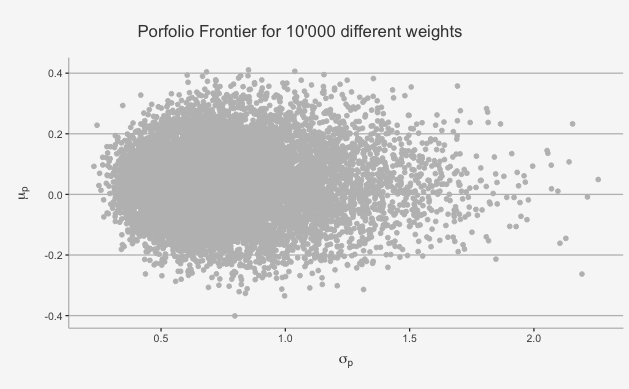
\includegraphics[width=0.8\linewidth]{attainable_port.png}
\caption{Feasible Portfolio}
\label{fig1}
\end{figure}
\end{frame}
%------------------------------------------------
\begin{frame}
\frametitle{Portfolio Performance}
\framesubtitle{Efficient Frontier}
\begin{figure}[H]
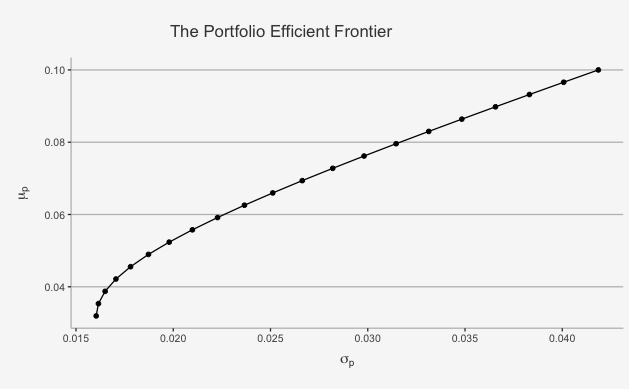
\includegraphics[width=0.8\linewidth]{EF.png}
\caption{Efficient Frontier}
\label{fig2}
\end{figure}
\end{frame}
%------------------------------------------------
%------------------------------------------------
%------------------------------------------------
\section{Conclusion}
\begin{frame}
\frametitle{Conclusion}
\begin{block}{Conclusion 1}
Among the 30 kinds of assets, 8 assets do not have inflation-hedging effects, including \textbf{four commodity futures}, Soybean Meal, Fuel Oil, Rebar, Wire Rod, \textbf{three industry stocks}, Energy, Main Consumption, and Telecommunication services, and \textbf{first-tier real estate}. The remaining 22 assets are chosen to construct the portfolio.
\end{block}
\end{frame}
%------------------------------------------------
\begin{frame}
\frametitle{Conclusion}
\begin{block}{Conclusion 2}
The \textbf{minimum-variance} portfolio and the \textbf{tangency} portfolio are calculated without short-selling restrictions. \\
\smallskip
Investment in \textbf{real estate} plays a pivotal role in hedging inflation risks. Investors are recommended to short real estate in third-tier cities and long real estate in second-tier cities in China if there are no short-selling restrictions.\\
\end{block}
\end{frame}
%------------------------------------------------
%------------------------------------------------
%------------------------------------------------
\section{References}
\begin{frame} % Use [allowframebreaks] to allow automatic splitting across slides if the content is too long
\frametitle{References}

\begin{thebibliography}{99} % Beamer does not support BibTeX so references must be inserted manually as below, you may need to use multiple columns and/or reduce the font size further if you have many references
\footnotesize % Reduce the font size in the bibliography

\bibitem[1]{p1}
Attié, Alexander P and Shaun K Roache (2009)
\newblock Inflation hedging for long-term investors
\newblock \emph{IMF Working Papers} 2009, 90.

\bibitem[2]{p2}
Di, JP (2012)
\newblock Can real estate provide a hedge against inflation evidence from Chinese mainland
\newblock \emph{Chinese Real Estate} 2, 10–17.

\bibitem[3]{p3}
Engsted, Tom and Carsten Tanggaard (2002)
\newblock The relation between asset returns and inflation at short and long horizons
\newblock \emph{Journal of International Financial Markets, Institutions and Money} 12(2), 101–118.

\bibitem[4]{p4}
Fama, Eugene F. and G.William Schwert (1977)
\newblock Asset returns and inflation
\newblock \emph{Journal of Financial Economics} 5(2), 115–146.

\end{thebibliography}
\end{frame}
%------------------------------------------------
\begin{frame} % Use [allowframebreaks] to allow automatic splitting across slides if the content is too long
\frametitle{References}

\begin{thebibliography}{99} % Beamer does not support BibTeX so references must be inserted manually as below, you may need to use multiple columns and/or reduce the font size further if you have many references
\footnotesize % Reduce the font size in the bibliography

\bibitem[5]{p5}
Levin, Eric J, A Montagnoli, and RE Wright (2006)
\newblock Short-run and long-run determinants of the price of gold
\newblock \emph{World Gold Council}

\bibitem[6]{p6}
Qin, S, CY Qin, and RX Chen (2004)
\newblock The optimal portfolios model with inflation rate
\newblock \emph{Systems Engineering Theory Methodology Application} 13(4), 316–319.

\bibitem[7]{p7}
Rapach, David E (2002)
\newblock The long-run relationship between inflation and real stock prices
\newblock \emph{Journal of Macroeconomics} 24(3), 331–351.

\bibitem[8]{p8}
Yu, Mei et al. (2015)
\newblock A Study on the Optimal Portfolio Strategies Under Inflation
\newblock \emph{Journal of Systems Science and Information} 3(2), 111–132.

\end{thebibliography}
\end{frame}
%------------------------------------------------
%------------------------------------------------
\begin{frame}[plain]
\begin{center}{\Huge Thanks for your time}\\
\bigskip
\bigskip % Vertical whitespace
{\LARGE Q\&A}
\end{center}
\end{frame}
%------------------------------------------------
\end{document} 